\documentclass[,man,floatsintext]{apa6}
\usepackage{lmodern}
\usepackage{amssymb,amsmath}
\usepackage{ifxetex,ifluatex}
\usepackage{fixltx2e} % provides \textsubscript
\ifnum 0\ifxetex 1\fi\ifluatex 1\fi=0 % if pdftex
  \usepackage[T1]{fontenc}
  \usepackage[utf8]{inputenc}
\else % if luatex or xelatex
  \ifxetex
    \usepackage{mathspec}
  \else
    \usepackage{fontspec}
  \fi
  \defaultfontfeatures{Ligatures=TeX,Scale=MatchLowercase}
\fi
% use upquote if available, for straight quotes in verbatim environments
\IfFileExists{upquote.sty}{\usepackage{upquote}}{}
% use microtype if available
\IfFileExists{microtype.sty}{%
\usepackage{microtype}
\UseMicrotypeSet[protrusion]{basicmath} % disable protrusion for tt fonts
}{}
\usepackage{hyperref}
\hypersetup{unicode=true,
            pdftitle={Instance theory predicts information theory: Episodic uncertainty as a determinant of keystroke dynamics},
            pdfauthor={Matthew J. C. Crump, Walter Lai, \& Nicholaus P. Brosowsky},
            pdfkeywords={Instance Theory, Information Theory, Entropy, Uncertainty, Typing, Performance},
            pdfborder={0 0 0},
            breaklinks=true}
\urlstyle{same}  % don't use monospace font for urls
\usepackage{graphicx,grffile}
\makeatletter
\def\maxwidth{\ifdim\Gin@nat@width>\linewidth\linewidth\else\Gin@nat@width\fi}
\def\maxheight{\ifdim\Gin@nat@height>\textheight\textheight\else\Gin@nat@height\fi}
\makeatother
% Scale images if necessary, so that they will not overflow the page
% margins by default, and it is still possible to overwrite the defaults
% using explicit options in \includegraphics[width, height, ...]{}
\setkeys{Gin}{width=\maxwidth,height=\maxheight,keepaspectratio}
\IfFileExists{parskip.sty}{%
\usepackage{parskip}
}{% else
\setlength{\parindent}{0pt}
\setlength{\parskip}{6pt plus 2pt minus 1pt}
}
\setlength{\emergencystretch}{3em}  % prevent overfull lines
\providecommand{\tightlist}{%
  \setlength{\itemsep}{0pt}\setlength{\parskip}{0pt}}
\setcounter{secnumdepth}{0}
% Redefines (sub)paragraphs to behave more like sections
\ifx\paragraph\undefined\else
\let\oldparagraph\paragraph
\renewcommand{\paragraph}[1]{\oldparagraph{#1}\mbox{}}
\fi
\ifx\subparagraph\undefined\else
\let\oldsubparagraph\subparagraph
\renewcommand{\subparagraph}[1]{\oldsubparagraph{#1}\mbox{}}
\fi

%%% Use protect on footnotes to avoid problems with footnotes in titles
\let\rmarkdownfootnote\footnote%
\def\footnote{\protect\rmarkdownfootnote}


  \title{Instance theory predicts information theory: Episodic uncertainty as a determinant of keystroke dynamics}
    \author{Matthew J. C. Crump\textsuperscript{1,2}, Walter Lai\textsuperscript{1}, \& Nicholaus P. Brosowsky\textsuperscript{2}}
    \date{}
  
\shorttitle{Episodic Uncertainty and Performance}
\affiliation{
\vspace{0.5cm}
\textsuperscript{1} Brooklyn College of the City University of New York\\\textsuperscript{2} The Graduate Center of the City University of New York}
\keywords{Instance Theory, Information Theory, Entropy, Uncertainty, Typing, Performance\newline\indent Word count: 5946}
\usepackage{csquotes}
\usepackage{upgreek}
\captionsetup{font=singlespacing,justification=justified}

\usepackage{longtable}
\usepackage{lscape}
\usepackage{multirow}
\usepackage{tabularx}
\usepackage[flushleft]{threeparttable}
\usepackage{threeparttablex}

\newenvironment{lltable}{\begin{landscape}\begin{center}\begin{ThreePartTable}}{\end{ThreePartTable}\end{center}\end{landscape}}

\makeatletter
\newcommand\LastLTentrywidth{1em}
\newlength\longtablewidth
\setlength{\longtablewidth}{1in}
\newcommand{\getlongtablewidth}{\begingroup \ifcsname LT@\roman{LT@tables}\endcsname \global\longtablewidth=0pt \renewcommand{\LT@entry}[2]{\global\advance\longtablewidth by ##2\relax\gdef\LastLTentrywidth{##2}}\@nameuse{LT@\roman{LT@tables}} \fi \endgroup}
\setlength{\parskip}{0.25cm plus4mm minus3mm}

\authornote{We dedicate this manuscript to Douglas J. K. Mewhort (1942 - 2019), who's work inspired our own. This entire manuscript is reproducible, and the data and analysis scripts are available at \url{https://osf.io/bdnqr/} (Crump, Lai, \& Brosowsky, 2018). This work was supported by a grant from NSF (1353360) to Matthew Crump.

Correspondence concerning this article should be addressed to Matthew J. C. Crump, Brooklyn College of CUNY, 2900 Bedford Avenue, Brooklyn, NY, 11210. E-mail: \href{mailto:mcrump@brooklyn.cuny.edu}{\nolinkurl{mcrump@brooklyn.cuny.edu}}}

\abstract{
How does prior experience shape skilled performance in structured environments? We use skilled typing of natural text to evaluate correspondence between performance (keystroke timing) and structure in the environment (letter uncertainty). We had \textasciitilde{}350 typists copy-type english text. We reproduced Ostry's (1983) analysis of interkeystroke interval as a function of letter position and word length, that showed prominent first-letter and mid-word slowing effects. We propose a novel account that letter position and word length effects on keystroke dynamics reflect informational uncertainty about letters in those locations, rather than resource limited planning/buffering processes. We computed positional uncertainty for letters in all positions of words from length one to nine using Google's n-gram database. We show that variance in inter-keystroke interval by letter position and word length tracks natural variation in letter uncertainty. Finally, we provide a model showing how a general learning and memory process could acquire sensitivity to patterns of letter uncertainty in natural english. In doing so, we draw an equivalence between Logan's (1988) instance theory of automatization and Shannon's measure of entropy (H) from information theory. Instance theory's predictions for automatization as a function of experience follow exactly the uncertainty in the choice set being automatized. As a result, instance theory stands as a general process model explaining how context-specific experiences in a structured environment tune skilled performance.


}

\begin{document}
\maketitle

\hypertarget{public-significance-statement}{%
\section{Public Significance Statement}\label{public-significance-statement}}

We used skilled typing as a task to investigate underlying cognitive processes involved in skilled action sequencing. In general, the major finding was that variation in typing performance at the letter level (how fast or you slow a typist types particular letters) can be well-explained by the statistics of letter occurrences as they appear in natural text. Our findings have implications for cognitive theory, and may also be useful for guiding typing curriculum for training typing skill.

\newpage

\hypertarget{introduction}{%
\section{Introduction}\label{introduction}}

Theories of cognitive processes run along a continuum from specific to general. On one extreme, cognitive phenomena are explained in terms of dedicated modules (Fodor, 1983) that give rise to cognition by the specialized principles of their internal processing architecture. On the other extreme, cognitive phenomena are explained in terms of general learning and memory processes (Jacoby \& Brooks, 1984; Kolers \& Roediger, 1984; Rumelhart \& McClelland, 1986) that give rise to cognition by applying general processing principles to experience in structured environments (Clark, 2008). Valid theories produce explanations of phenomena by deduction from their processing assumptions, and then compete with other valid theories on the basis of parsimony. When phenomena are explained by general processes, specialized accounts remain sufficient, but not necessary; and, vice versa. We continue in this tradition by proposing and validating a general process account of keystroke dynamics in skilled typing performance. We show that keystroke dynamics can emerge from a general memory process sensitive to structure (uncertainty) in the natural language environment.

We identified the following pre-requisites as necessary for our approach. We assume that performance is driven by learning processes sensitive to the structure in the environment. So, we require a tool for describing the structure of environmental inputs. And, we require a model that articulates how learning about the structure of an environment produces performance. Finally, we require a task where the relation between performance and a structured environment can be measured. We use information theory (Shannon \& Weaver, 1949) to measure the structure of the letters that typists' type, instance theory (Logan, 1988) to model how typists' performance is shaped by the typing environment, and the task of continuous typing (Logan \& Crump, 2011) to measure keystroke dynamics as a function of the structure in the typing environment.

There are many typing phenomena to explain (Salthouse, 1986), and several existing models of typing (Heath \& Willcox, 1990; John, 1996; Logan, 2018; Rumelhart \& Norman, 1982; Wu \& Liu, 2008). Our goal here was not to provide another general model of typing, and we expect that our model will fail to explain many aspects of typing performance. Instead, we focus our efforts empirically and theoretically as follows. Empirically, we examine whether typing performance is constrained by structure in the natural language. Theoretically, we propose a general processing account that predicts how structure in the natural language should constrain typing performance. These aims contribute to the broader goals (beyond the scope of this paper) of determining whether specialized or general accounts are necessary or sufficient to explain typing performance, and then adjudicating between them.

We focused on two typing phenomena, the word-initiation/first-letter slowing effect, and the mid-word slowing effect, which are both observed in continuous copy-typing of words presented in sentences. First-letter slowing refers to longer keystroke times for letters in the first position of a word compared to other letters. Mid-word slowing refers to an inverted U shaped pattern, with longer interkeystroke intervals (IKSIs) for letters in the middle of a word compared to letters at the beginning and ending of a word. First-letter and mid-word slowing were clearly demonstrated by Ostry (1983), who showed systematic effects of letter position and word length on IKSIs.

We chose these phenomena for two reasons. First, both phenomena have been explained in terms of specialized processes, and it remains unclear whether those accounts are necessary to explain the phenomena. Second, we have not found work replicating Ostry's (1983) results, and Salthouse (1986) suggested that effects of word length do not systematically influence interkeystroke intervals, so the effects of letter position and word length on interkeystroke interval remain unclear.

First-letter slowing has been explained in terms of planning and buffering processes associated with typing a whole word (Salthouse, 1986). For example, the time associated with retrieving a motor program for a word, parsing the word into letters, planning the sequence, or initiating the execution of the sequence after it is buffered, could cause the first letter in a word to be produced more slowly than other letters. Mid-word slowing has been explained in terms of rising interference from ongoing sequencing, or from micro-planning of syllables that occur in the middle of words (Will, Nottbusch, \& Weingarten, 2006). These explanations rely on largely unspecified planning and execution processes.

To develop an alternative, we entertained a simple question: are more predictable letters typed faster than less predictable letters? More specifically, we wondered whether natural variation in letter uncertainty as a function of letter position and word length would magically (in the sense of Miller, 1956) correspond to the observed variation in interkeystroke intervals as a function of letter position and word length. Such a demonstration would license consideration of how a general learning process sensitive to letter uncertainty could explain effects of letter position and word length on interkeystroke intervals.

Prior work shows that typists are sensitive to structures in the text the type. For example, IKSIs are correlated with letter and bigram frequency (Behmer \& Crump, 2017; Grudin \& Larochelle, 1982; Salthouse, 1984; Terzuolo \& Viviani, 1980), trigram frequency (Behmer \& Crump, 2017), and word frequency (Vinson, 2017). Individual keystroke times are influenced by the immediate letter context in which they occur (Gentner, 1982; Shaffer, 1973). IKSIs are also influenced by orthographic structure (Massaro \& Lucas, 1984; Pinet, Ziegler, \& Alario, 2016; Will et al., 2006). Finally, IKSIs are much shorter for letter strings from a natural language, compared to random letter strings (Behmer \& Crump, 2017; Shaffer \& Hardwick, 1968). These demonstrations suggest that typing performance is partly determined by a learning process sensitive to structure inherent to natural texts.

Following Shannon and Weaver (1949), we use information theory as a tool to measure structure in natural texts. The summary statistic H measures the entropy or uncertainty in any discrete probability distribution of a set of items. H goes to 0 for distributions that are perfectly predictable (e.g., when one item occurs 100\% of the time). H goes to its maximum value for distributions that are completely unpredictable, fully entropic, or maximally uncertain (e.g., when all items occur with equal probability). Shannon's H is defined as:

\(H = -\sum p \log_2 p\)

where, p is the probability of occurrence for each item in a given distribution. H is the number of bits needed to represent the distribution. To apply this to letter uncertainty, consider the set of the 26 lowercase letters from a to z. For this set, H can range from 0 to \textasciitilde{}4.7. H approaches 4.7 as letter probabilities approach a uniform distribution, indicating all letters are equiprobable, \(H = -\sum \frac{1}{26} \log_2 \frac{1}{26} = 4.7004\). H by definition is less than 4.7 for all unequal letter probability distributions, where some letters occur with higher or lower probabilities than others.

Most important, H can be calculated for any letter probability distribution. For example, if separate letter probability distributions for every letter position across words of every length in natural English text could be obtained, then the letter uncertainty for each position by word length could be calculated; and, correspondence between letter uncertainty and interkeystroke intervals as a function of letter position and word length could be evaluated.

Our empirical question also ties into the well known application of information theory to choice-reaction time performance. For example, Hick (1952), and Hyman (1953) showed that choice reaction time, which was known to increase as a function of set-size, increases linearly as a function of choice uncertainty in the set (measured by H), rather than set-size per-say. Although there are numerous exceptions to the Hick-Hyman law (for a review see, Proctor \& Schneider, 2018), we are not aware of any work that has determined whether typing performance (a continuous 26-AFC choice-task, assuming lower case for convenience) depends on letter uncertainty. If typing performance does depend on letter uncertainty, then a model based explanation of the dependency is required.

\hypertarget{overview-of-present-study}{%
\subsection{Overview of present study}\label{overview-of-present-study}}

We first reproduce Ostry's (1983) analysis of interkeystroke intervals as a function of letter position and word length. We used the dataset collected by Behmer and Crump (2017), who had 346 typists copy type five paragraphs of natural English text. Then we estimated letter uncertainty in natural English for each letter position in words of different lengths. We used letter frequency counts from Google's Ngram project provided by Peter Norvig, who made tables of separate letter frequency distributions as a function of letter position and word length. We converted these frequency distributions to letter probability distributions to calculate letter uncertainty (H) for each letter position in words of length one to nine. We show that natural variation in letter uncertainty can explain large portions of variance in interkeystroke intervals as a function of letter position and word length; and, we develop a formal model of these results using the instance theory of automatization (Logan, 1988). In the general discussion we evaluate whether planning accounts of first-letter and mid-word slowing remain necessary in light of the present findings.

\hypertarget{methods}{%
\section{Methods}\label{methods}}

We re-analyzed copy-typing data from 346 participants who completed an online typing task (Behmer \& Crump, 2017). The procedure was approved by the institutional review board at Brooklyn College of the City University of New York. Participants were recruited through Amazon's Mechanical Turk, and used a web-browser to copy-type five paragraphs from the Simple English Wiki (average 131 words each), and perform additional typing tasks (such as typing random letter strings and english-like nonwords). See the supplementary materials for additional details about the design.

\hypertarget{data-analysis-and-pre-processing}{%
\subsection{Data analysis and pre-processing}\label{data-analysis-and-pre-processing}}

We used R for all the analyses, figure generation, model simulation, and to write this paper as a reproducible manuscript. All of the code necessary to reproduce this manuscript can be found at \url{https://osf.io/bdnqr/}.

For each subject, we applied the following pre-processing steps to their performance on the five English pargraphs. We included IKSIs only for keystrokes involving a lower case letter, and only for correct keystrokes that were preceded by a correct keystroke. Outlier IKSIs were removed for each subject, on a cell-by-cell basis, using the Van Selst and Jolicoeur (1994) non-recursive moving criterion procedure, which eliminated approximately 3\% of IKSIs from further analysis.

\hypertarget{results}{%
\section{Results}\label{results}}

\hypertarget{typing-performance}{%
\subsection{Typing Performance}\label{typing-performance}}

\begin{figure}
\centering
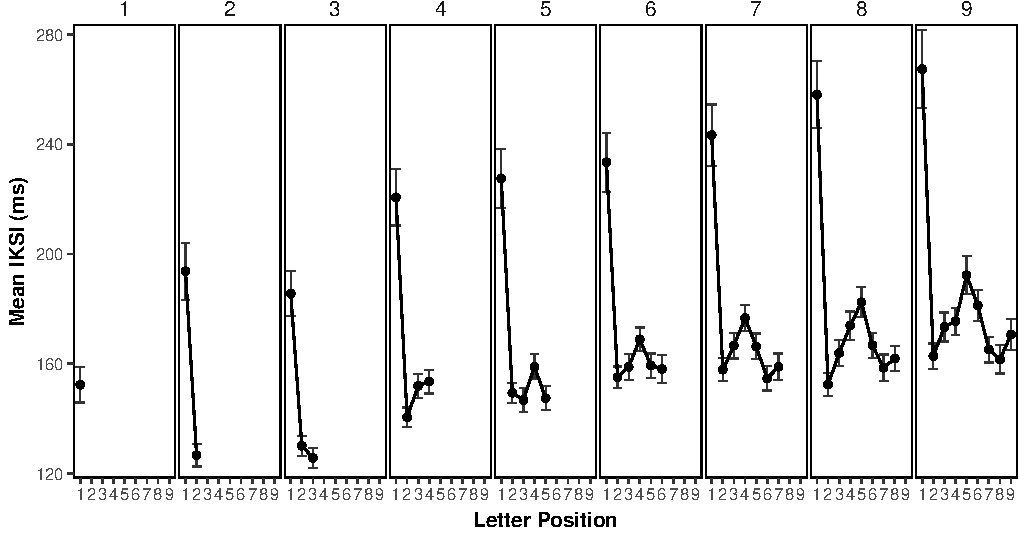
\includegraphics{v2-manuscript_files/figure-latex/figure1-1.pdf}
\caption{\label{fig:figure1}Mean interkeystroke intervals (ms) as a function of word length (panels) and letter position. Error bars represent 95\% confidence intervals around the mean typing speed.}
\end{figure}



For each subject, we calculated mean IKSIs as a function of letter position and word length (see Figure \ref{fig:figure1}). Visual inspection of \ref{fig:figure1} shows that mean IKSIs for first positions were generally longer than mean IKSIs for other positions; and, that mean IKSIs in middle positions were generally longer than mean IKSIs in surrounding positions.

\begin{figure}
\centering
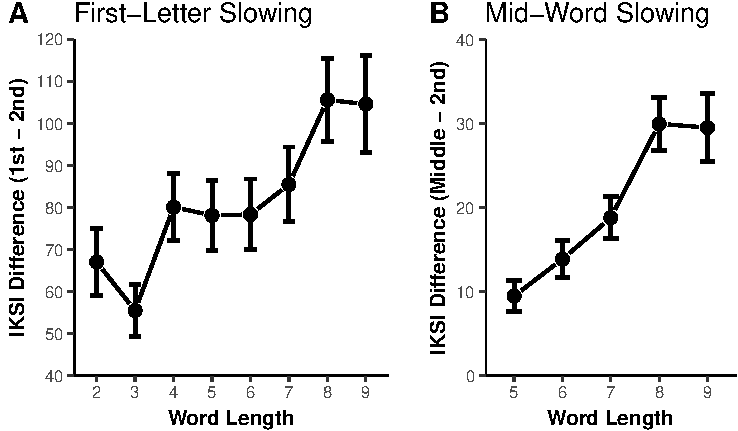
\includegraphics{v2-manuscript_files/figure-latex/figure2-1.pdf}
\caption{\label{fig:figure2}Panel A shows first-letter slowing as mean IKSI (ms) differences between 2nd and 1st letter positions as a function of word length. Panel B shows mean IKSI differences (ms) between the middle and 2nd letter positions as a function of word length. The middle position indicates the peak middle letter position from each word length. Error bars represent 95\% confidence intervals around the mean difference scores.}
\end{figure}



To assess first-letter slowing, we compared first versus second position IKSIs for words with two to nine letters (see Figure \ref{fig:figure2}A). We submitted mean IKSIs to a 2x8 repeated measures ANOVA with letter position (1st and 2nd) and word length (2, 3, 4, 5, 6, 7, 8, and 9) as factors. We found a significant main effect of letter position, \(F(1, 345) = 381.42\), \(\mathit{MSE} = 24325.26\), \(p = 9.78e-58\), \(\hat{\eta}^2_\textit{p} = 0.53\), showing slower typing speeds in the first position (\textit{M} = 229ms) as compared to the second (\textit{M} = 147ms). We also found a significant main effect of word length, \(F(7, 2415) = 496.38\), \(\mathit{MSE} = 590.11\), \(p = 0\), \(\hat{\eta}^2_\textit{p} = 0.59\), and an interaction between word length and letter position, \(F(7, 2415) = 110.07\), \(\mathit{MSE} = 457.3\), \(p = 2.69e-140\), \(\hat{\eta}^2_\textit{p} = 0.24\). Generally speaking, the first-letter slowing effect increased with longer words, plateauing at word length eight.

To assess mid-word slowing, we adopted the same procedure as Ostry (1983): From each word length, we selected the position with the longest reaction time between positions three through nine as the \enquote{middle}. We then compared typing performance from the middle position to the second position across words with five to nine letters (see Figure \ref{fig:figure2}B). We submitted mean IKSIs to a 2x4 repeated measures ANOVA with letter position (2nd and middle) and word length (5,6,7, and 8) as factors. We found a significant main effect of letter position, \(F(1, 345) = 381.42\), \(\mathit{MSE} = 24325.26\), \(p = 9.78e-58\), \(\hat{\eta}^2_\textit{p} = 0.53\), showing slower typing speeds for the middle position (\textit{M} = 176ms) as compared to the second position (\textit{M} = 156ms). We also found a significant main effect of word length, \(F(7, 2415) = 496.38\), \(\mathit{MSE} = 590.11\), \(p = 0\), \(\hat{\eta}^2_\textit{p} = 0.59\), and a significant interaction between word length and letter position, \(F(7, 2415) = 110.07\), \(\mathit{MSE} = 457.3\), \(p = 2.69e-140\), \(\hat{\eta}^2_\textit{p} = 0.24\). As with first-letter slowing, the mid-word slowing effect increased as a function of word length and plateaued at word length eight.

\hypertarget{letter-uncertainty-by-position-and-word-length}{%
\subsection{Letter Uncertainty by position and word length}\label{letter-uncertainty-by-position-and-word-length}}

The primary question of interest was whether natural variation in letter uncertainty explains variance in mean IKSI by position and word length. We estimated letter uncertainty by position and word length from Google's Ngram database (\url{https://books.google.com/ngrams}), which provides frequency counts of letters and words occurring in Google's corpus of millions of digitized books. Letter frequency counts for letters a to z, for each position in words from length one to nine, were obtained from Peter Norvig's website (\url{http://norvig.com/mayzner.html}).

For each of the 45 letter frequency distributions (position x word length), we computed Shannon's H (entropy) to quantify letter uncertainty. We converted each letter frequency distribution to a probability distribution then calculated H for each distribution. Figure \ref{fig:figure3} displays estimates of letter uncertainty (H) as a function of letter position and word length (unigram: circle/solid line). We discuss the H values for the bigram estimates in a following section.

\begin{figure}
\centering
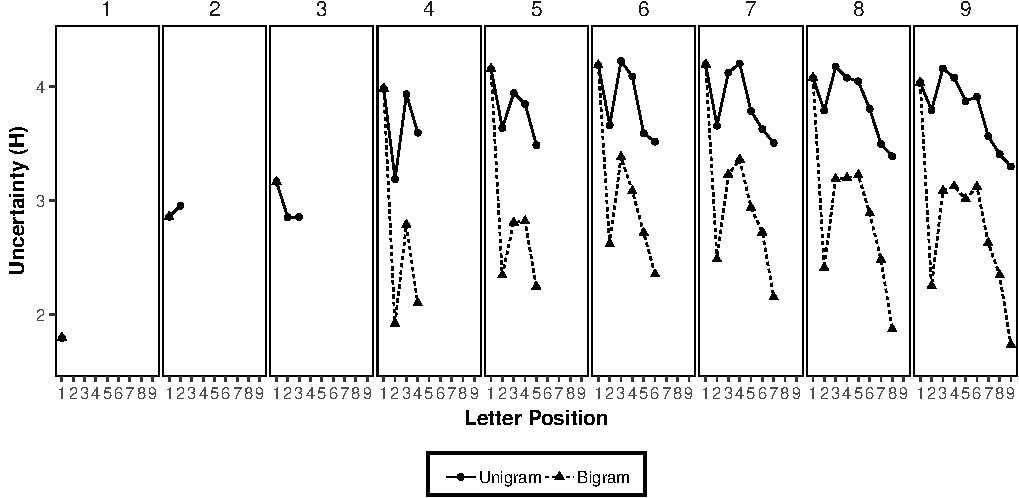
\includegraphics{v2-manuscript_files/figure-latex/figure3-1.pdf}
\caption{\label{fig:figure3}Letter uncertainty (H, from Google n-gram corpus) for each letter position as a function of word length and calculated using unigram position probabilities (square) or conditionalized using N-1 bigram letter probabilities (triangle).}
\end{figure}



To our knowledge this a novel analysis of how letter uncertainty in natural English varies by word length and position. We were interested in whether letters appearing the first position of words would have larger H values than letters in other positions; and, whether letters appearing in the middle of words would have larger H values than letters appearing around the surrounding positions. Visual inspection of the graph shows letters in the first position have generally larger H values than other positions, and letters in the middle positions have generally larger H values than letters surrounding the middle position. This suggests that natural variation of letter uncertainty across position and word in English may account for aspects of the first-letter and mid-word slowing phenomena in typing.

\hypertarget{letter-uncertainty-and-mean-iksi}{%
\subsection{Letter Uncertainty and Mean IKSI}\label{letter-uncertainty-and-mean-iksi}}

If the Hick-Hyman law applied to continuous typing we would expect a neat linear relationship between mean IKSIs and letter uncertainty. Figure \ref{fig:figure4} shows a plot of mean IKSIs taken from all positions and word lengths against letter uncertainty (panel A).

\begin{figure}
\centering
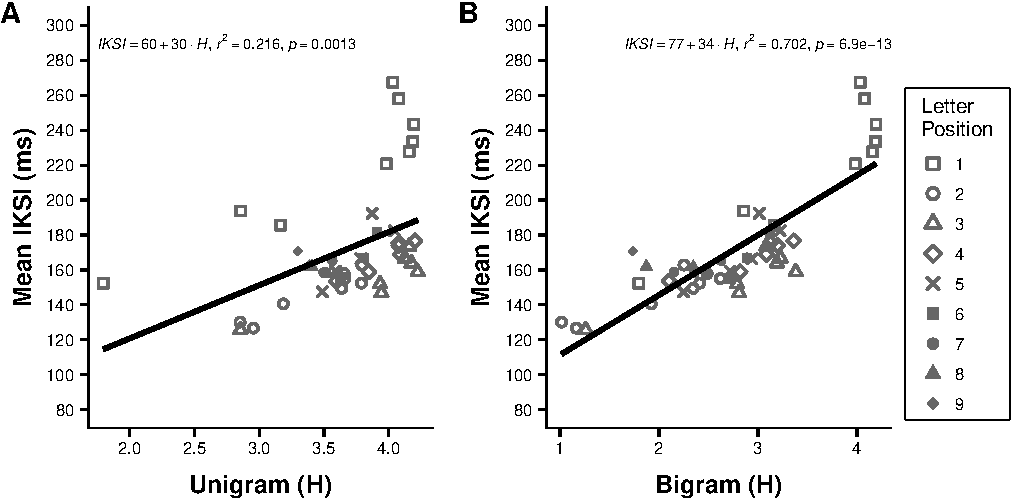
\includegraphics{v2-manuscript_files/figure-latex/figure4-1.pdf}
\caption{\label{fig:figure4}Mean interkeystroke interval (ms) for each letter position and word length is plotted as a function of letter uncertainty (H) calculated using unigram position probabilities (A) or conditionalized using N-1 bigram probabilities (B).}
\end{figure}



A linear regression with group mean IKSIs (collapsed over subjects) as the dependent variable, and letter uncertainty as the independent variable showed a significant positive trend, F(1, 43) = 11.82, p = 0.0013, \(R^2 =\) 0.22 (IKSI = 59.75 \(+\) 30.49 \(* H\)). We also conducted separate linear regressions for each subject and found similar results. For example, the mean correlation was r = 0.67 (SE = 0.0089); mean \(R^2\) = 0.48 (SE = 0.0091); and mean p = 0.021 (SE = 0.0058).

\hypertarget{interim-discussion}{%
\subsection{Interim Discussion}\label{interim-discussion}}

We can conclude that letter uncertainty as a function of position and length explains a small amount variation in mean IKSIs during continuous typing. The present analysis does not provide strong evidence that a process sensitive to letter uncertainty causes both first-letter and mid-word slowing. For example, all of the first position mean IKSIs are longer than mean IKSIs for other positions at comparable levels of letter uncertainty. And, a linear regression on the group mean IKSIs including letter uncertainty and position (first letter vs.~other letter) as independent variables explains much more variance, \(R^2\) = 0.86, p \textless{} .001, than the regression only including letter uncertainty.

This pattern invites a dual-process interpretation. For example, first-letter slowing could be explained by a planning process that increases first position IKSIs as a function of word length. Longer words have more letters, thus plan construction and buffering is assumed to take more time before sequence production begins. At the same time, the finding that letter uncertainty does explain some variance in mean IKSI across position suggests that sequence production is also influenced by a process sensitive to letter uncertainty.

\hypertarget{letter-uncertainty-by-position-word-length-and-n-1-letter-identity}{%
\subsection{Letter Uncertainty by position, word length, and n-1 letter identity}\label{letter-uncertainty-by-position-word-length-and-n-1-letter-identity}}

Determining whether first-letter and mid-word slowing could emerge from a process sensitive to letter uncertainty depends on how letter uncertainty is calculated. Letter uncertainty can be calculated from any discrete probability distribution of letters. In the previous section we somewhat arbitrarily calculated letter uncertainty separately for each letter position in words of length one to nine. However, the number of alternative schemes is vast. For example, we could further conditionalize position by word length probability distributions by the identities of letters occurring in any position n-1 to n-x, or n+1 to n+y of a specific position. Furthermore, we could conditionalize letter distributions upon any permissible number of preceding or succeeding n-grams (groups of letters).

Although an exhaustive calculation of letter uncertainty is beyond the scope of this paper, we nevertheless took one further step and calculated letter uncertainty by position and word length, conditionalizing upon n-1 letter identity (referred to as bigram uncertainty in figure \ref{fig:figure3}). Fortunately, Norvig (\url{http://norvig.com/mayzner.html}) also provided bigram frequency counts from the Google Ngram corpus as a function of position and word length. We calculated letter uncertainty in the following manner. First position letters have no preceding letter, so H as a function of word length was identical to our prior calculation. For letters in positions two to nine, for all word lengths, we calculated H for every n-1 letter identity, multipled each H by the overall probability of each letter in the n-1 position\footnote{Thanks to reviewer Michael Masson for suggesting we weight H for each n-1 letter distribution as a function of n-1 letter probability.}, and then took the sum of the Hs to create a weighted mean H. For example, the second position of a two-letter word has a maximum of 26 letter probability distributions, one for each possible n-1 letter (a to z). We calculated H for all n-1 distributions, weighted the Hs by the probabilities of each n-1 letter, then took the sum of the weighted Hs as the mean letter uncertainty for that position. Panel B of figure \ref{fig:figure3} shows mean H conditionalized by n-1 letter identity, as a function of letter position and word length.

Unsurprisingly, letter uncertainty is decreased when n-1 letter identity is known. Compared to the unigram uncertainty measures, we see that H for letters in positions two to nine is much lower when n-1 letter identity is taken into account. More important, the pattern of H in Figure \ref{fig:figure3} much more closely resembles the pattern of mean IKSIs in Figure \ref{fig:figure1}.

Figure \ref{fig:figure4}B displays a scatterplot of mean IKSIs as a function of letter uncertainty conditionalized by letter n-1 identity across positions and word length. A linear regression on mean IKSIs using the new measure of letter uncertainty as the independent variable showed a strong positive relationship, F(1, 43) = 101.48, p \textless{} 0.001, \(R^2 =\) 0.70 (IKSI = 77.00 \(+\) 34.31 \(*H\)). Including n-1 letter identity into the estimate of letter uncertainty clearly allowed H to explain much more variance in mean IKSIs compared to the previous measure of H.

Finally, we conducted a linear regression that included letter position (first position vs.~other position) along with H (conditionalized by n-1 letter identity, position, and length). That model explained the largest amount of variance, \(R^2\) = 0.88, p \textless{} .001, compared to all previous models. We discuss this finding with respect to explanations of first-letter and mid-word slowing in the general discussion.

\hypertarget{an-instance-based-model}{%
\section{An instance-based model}\label{an-instance-based-model}}

We have shown that variation in mean IKSIs as a function of letter position and word length can be well explained by natural variation in letter uncertainty conditionalized by letter n-1 identity, position, and word length. The correlational nature of this evidence prevents any causal conclusions about how variation in mean IKSI might be caused by variation in uncertainty. In the general discussion we discuss further steps for future work to establish causality by experiment. In addition to empirical work, it is also necessary to provide a working process model that articulates how variation in letter uncertainty could cause variation in mean IKSIs. In this section, we establish theoretical plausibility by showing that letter uncertainty influences on performance can be explained in terms of Logan's (1988) instance theory of automatization.

\hypertarget{prior-modeling-work}{%
\subsection{Prior modeling work}\label{prior-modeling-work}}

Before describing our modeling approach, we first point out that instance-based models have already been used to explain reaction time phenomena that depend on informational uncertainty. For example, Jamieson and Mewhort (2009) showed that a variant of MINERVA 2 (Hintzman, 1984, 1986, 1988), an instance-based theory of memory, can explain performance in a variety of serial reaction time tasks (e.g., Nissen \& Bullemer, 1987), and explain the dependence of choice-reaction times on the Hick-Hyman law (Hick, 1952; Hyman, 1953). Both are critical antecedents to the present work, and we discuss each in turn.

In a typical serial reaction time task, participants identify the location of a stimulus that could appear in one of four locations as quickly and accurately as possible. In this task, performance depends on the predictability of the target locations. When the location of the stimuli vary randomly from trial-to-trial, little to no learning is observed (mean RTs do not decrease much with practice. When the location of the stimuli follows a hidden repeating sequence, learning is observed (mean RTs get much shorter with practice). Jamieson and Mewhort (2009) conducted a version of the SRT using probabilistic sequences that varied in informational uncertainty. They found that people learned more as the uncertainty in the sequence decreased (became more predictable). Furthermore, they modeled those results with MINERVA 2, thereby demonstrating that an instance-based model learns about sequences as a function of the amount of information in the sequence. There are clear parallels between typing and the SRT task, in that typing is a real-world task where people learn to produce sequences that vary in their infomational uncertainty.

Next, Jamieson and Mewhort (2009) showed the same model can account for performance in a choice-reaction time task that varies stimulus uncertainty. In particular, they applied the model to a classic design by Hyman (1953), and showed that it could simulate the major finding that mean reaction was a linear function of informational uncertainty in sets of choices.

So, Jamieson and Mewhort (2009) have already developed an instance-based explanation of how variation in mean RT for a set of items depends on the information (uncertainty) in the set. We assume that, in principle, we could have used their model to simulate the process of learning type letters as they occur in different letter positions and word lengths, and then evaluate whether the model also predicts that mean IKSIs would very as a function of letter uncertainty in those contexts. However, we chose to evaluate predictions from a different instance-based model (Logan, 1988), which allowed us to assess whether instance models that are computationally quite different, nevertheless produce similar predictions.

\hypertarget{modeling-uncertainty-with-the-instance-theory-of-automatization}{%
\subsection{Modeling uncertainty with the instance theory of automatization}\label{modeling-uncertainty-with-the-instance-theory-of-automatization}}

Logan's (1988) instance theory provides an account of how performance becomes automatized with practice. We will show that this instance theory is also sensitive to uncertainty in the sets of stimuli it encounters over practice. More specifically, we will draw an equivalence between instance theory and the information theoretic measure of H, and show that instance theory predictions for performance are nearly identical to H. As a result, instance theory, like MINERVA 2, becomes a process model of the Hick-Hyman law, which posits that reaction times are a linear function of the uncertainty in a choice set.

Instance theory models learning as a function of practice in terms of cue-driven retrieval of stored memory traces (like other global memory models, Eich, 1982; Hintzman, 1988; Humphreys, Pike, Bain, \& Tehan, 1989). A new unique trace is preserved in memory every time a response is given to a stimulus. When a familiar stimulus is encountered again, it automatically triggers the retrieval of all stored instances of the stimulus. The timing of the memory-based response to a current stimulus is treated as a race. Whichever memory trace is retrieved first wins the race. As a result, the memory-based reaction time to respond to a stimulus is determined by the retrieval time associated with the fastest memory trace for that stimulus. The retrieval times for every memory trace are assumed to vary, and can be sampled from any desired distribution.

In other words, instance theory models practice based performance speed-ups (power law of learning) in terms of sampling extreme values from a growing retrieval time distribution. As the number of memory traces grows, the range of the retrieval time distribution also grows, such that the minimum value of the distribution (shortest retrieval time) is more likely to be smaller for distributions with more than fewer memory traces. As a result, reaction times will tend to be shorter for more practiced than less practiced stimuli, because more practiced stimuli have a better chance of retrieving a fast memory response than less practiced stimuli.

\hypertarget{hyman-1953}{%
\subsection{Hyman (1953)}\label{hyman-1953}}

We first demonstrate that the instance theory of automatization can reproduce the results of Hyman (1953). Hyman ran three choice reaction-time experiments, all involving responding to one of eight lights with a learned vocal response for each light. Across experiments, the number of items, frequency of items, and sequential probability of items were systematically varied to produce many different choice sets with different amounts of uncertainty. Experiment 1 had eight conditions, varying the number of alternatives from 1 to 8. Within each condition, each alternative appeared equally often. Experiment 2 had eight conditions, each involving different numbers of alternatives, but within each condition specific items appeared with higher or lower probabilites than other items. Experiment 3 had eight conditions, each condition involved different numbers of alternatives, and the probability of specific items appearing depended on the identity of the previous item. Hyman calculated the information in bits (H) for each condition in each experiment, which ranged from 0 to 3 (see Hyman, 1953, for tables showing the probabilties of each item in each condition). Hyman showed that mean reaction time in each condition was a linear function of the number of bits for the choice set in each condition.

We conducted a simulation in R to model instance theory predictions for mean reaction time across all conditions in the three experiments (see supplementary materials or the repository for the code). Our approach to simulating instance theory predictions was to model reaction times for an average subject to respond to a specific item, given some number trials of practice with responding to the item. We treat all items as completely independent, such that when a particular stimulus is \enquote{presented}, it only retrieves traces specific to the history for that stimulus. In our implementation we assumed that memory retrieval times are sampled from a normal distribution with mean = 500, and standard deviation = 100. If a subject had practiced responding to an item 10 times, they would have 10 traces in memory, which would each have a particular retrieval time determined in our model by randomly sampling 10 numbers from the retrieval time distribution. The shortest retrieval time in that sample would be the model's reaction time after 10 practice trials. Of course, different subjects would have 10 randomly different memory traces, and the RT for the shortest RT in the sample will vary by chance. We were interested in estimating the average shortest retrieval time that would be expected given some amount of practice. Using Monte-carlo simulation, we found an estimate by creating 5,000 sets of samples (sample-size determined by amount of item-specific practice) from the retrieval time distribution, computing the minimum value in each sample, and then computing the mean of the minimum values across samples. Using this strategy we can compute expected mean reaction times for a stimulus based on how many times it has been practiced.

\begin{figure}
\centering
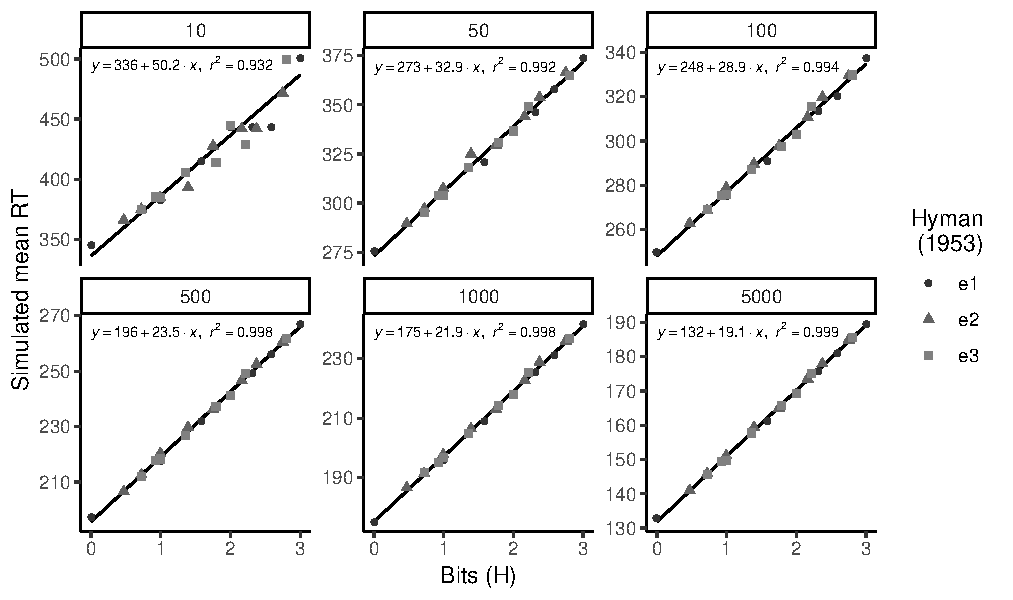
\includegraphics{figures/Hyman_figure.pdf}
\caption{\label{fig:figureHyman}Simulated mean reaction times for each condition from Hyman (1953), as a function of number of bits in each condition. Each facet represents amount of practice, from 10 to 5000 traces.}
\end{figure}



To extend this approach to the Hyman (1953) design, for each condition we computed the amount of practice for each item (given the overall amount of practice), found the average minimum retrieval time for each item, then averaged over the RT estimates for each item to get an estimate of the mean RT for the condition. Figure \ref{fig:figureHyman}, shows simulated mean reaction times for each condition as a function of bits in each condition. We evaluated the model across different amounts of practice (10,50,100,500,1000,5000). As is clear from the figure, instance theory predictions for mean RT in each condition are correlated with the amount of uncertainty in each condition; and the variance explained tends toward 1, as the amount of practice is increased.

This simulation extends prior work by Jamieson and Mewhort (2009), and shows that a wider range of instance models are capable of explaining the Hick-Hyman law. We suggest a novel finding here is the remarkably close fit between simulated mean RTs and H. In particular, it appears that instance theory makes exact predictions about H as practice tends toward a large n, and that simulated mean RTs are related to H by the constants in the regression lines.

\hypertarget{letter-uncertainty-as-a-function-of-position-word-length-and-n-1-letter-identity}{%
\subsection{Letter uncertainty as a function of position, word length, and n-1 letter identity}\label{letter-uncertainty-as-a-function-of-position-word-length-and-n-1-letter-identity}}

We now apply the same instance model to generate predictions for keystroke production times as a function of letter position, word length, and n-1 letter identity for typing natural English text. We treated all 26 letters that could possibly occur in any position for any word length, and preceded by any letter, as completely unique and independent stimuli. For example, the letter \enquote{a} occuring in all possible contexts was treated as separate stimuli, with separate trace counts. This assumes traces for specific letters are stored and retrieved in a context-dependent fashion (this assumption is consistent with a recent context-driven model of ordering in typing Logan, 2018; and with prior empirical work showing IKSIs for letters depend on surrounding letter context, Shaffer, 1973; Gentner, 1982). We modeled the structure of natural English using the letter probability distributions derived from Norvig's letter frequency counts by position and word length, and n-1 letter identity from Google's Ngram corpus.

For convenience, we assumed that the retrieval time distribution for each stimulus was sampled from a normal distribution with mean = 500, and standard deviation = 100. Using R, we sampled retrieval times for each stimulus from the normal distribution n times, where n was the current number of memory traces for a given letter, that would have been experienced with a particular frequency. Then we took the minimum value from the sampling distribution as the reaction time for that stimulus, given n amount of practice. We repeated this process 1000 times to estimate the expected mean reaction time (expected minimum retrieval time) for the given frequency value for each letter in the set. In this way, we estimated mean keystroke production times for every letter position across different word lengths, collapsed across letter n-1 identity.

Last, we evaluated model predictions across four practice intervals, shown in Figure \ref{fig:figure5} as 50, 100, 500 and 10000. These practice intervals refer to the total number of keystrokes typed. The individual letter frequencies for each practice interval (the number of traces stored for each letter) were determined by multiplying each letter probability by the total number of keystrokes in the practice interval. The source code for the model is available in the repository for this manuscript.

\begin{figure}
\centering
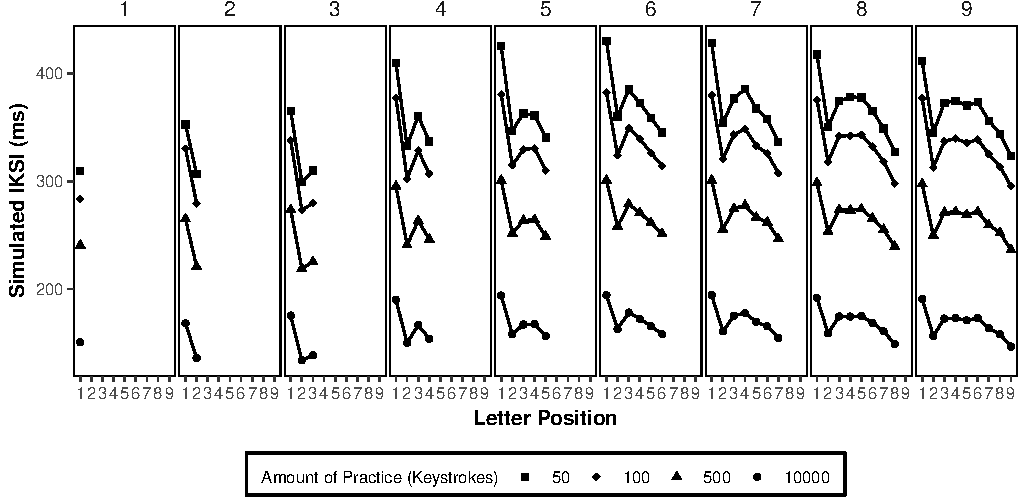
\includegraphics{v2-manuscript_files/figure-latex/figure5-1.pdf}
\caption{\label{fig:figure5}Each panel shows simulated mean IKSIs as a function of letter position and word length calculated using the conditionalized N-1 bigram probabilities. The numbers 50, 100, 500, and 10000 refer to increasing amounts of practice.}
\end{figure}



Figure \ref{fig:figure5} displays model predictions across increasing amounts of practice, for mean IKSIs as a function of letter position and word length simulated using the conditionalized letter n-1 probabilities. As expected, simulated mean IKSIs shorten with practice. More important, at each stage in practice, simulated mean IKSIs across letter and word length show the same pattern as measures of letter uncertainty (e.g., as seen in figure \ref{fig:figure3}.

\begin{figure}
\centering
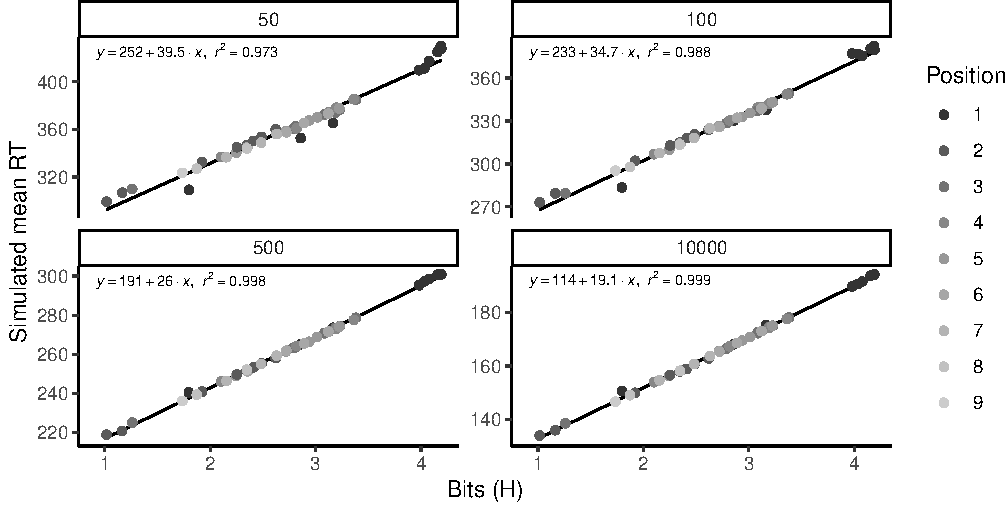
\includegraphics{v2-manuscript_files/figure-latex/figureInstanceBits-1.pdf}
\caption{\label{fig:figureInstanceBits}Each panel shows simulated mean IKSIs as a function of letter position and word length calculated using the conditionalized N-1 bigram probabilities. The numbers 50, 100, 500, and 10000 refer to increasing amounts of practice.}
\end{figure}



To show the relationship between simulated IKSI and H, we conducted linear regressions on simulated IKSIs using letter uncertainty as the independent variable. \ref{fig:figureInstanceBits} shows that letter uncertainty nearly perfectly explains the variance in simulated keystroke time, with \(R^2\) tending toward 1 with practice.

In summary, we have shown that the instance theory of automatization (Logan, 1988) provides an account of the Hick-Hyman law. In other words, instance theory predictions for mean reaction time for a set of independent choices depend on the amount of uncertainty, measured in terms of bits, in the set of choices. To state this differently again, the predictions for mean RTs for sets of items that vary in uncertainty, are identical to H, and but scaled by constant factors. We note that we did not ask how well instance theory predictions for mean typing time as a function of position and word length explain variance in the observed mean IKSIs. Although we could conduct that anlaysis, it would be redundant with the analysis using letter uncertainty values to explain variance in observed mean IKSIs, because instance theory converges on the same vector as the information theoretic measure of uncertainty.

\hypertarget{general-discussion}{%
\section{General Discussion}\label{general-discussion}}

Using data from a large N study of continuous typing performance, we reproduced Ostry's (1983) demonstration that mean interkeystroke interval systematically varies as a function of letter position and word length; and, reproduced evidence for first-letter and mid-word slowing effects. We proposed that variation in mean IKSI could be caused by a general learning process sensitive to letter uncertainty across letter position and word length. We calculated letter uncertainty in natural English from Google's large corpus of digitized text, and showed that it can explain variance in mean IKSI, especially when letter n-1 identity is included in the measure of uncertainty ( \(R^2\) = 0.70 ). Finally, we show that instance theory (Logan, 1988) can explain the Hick-Hyman law, and by extension, successfully models how a general learning and memory process could produce typing performance as a function of letter uncertainty.

\hypertarget{planning-versus-learning-about-letter-uncertainty}{%
\subsection{Planning versus learning about letter uncertainty}\label{planning-versus-learning-about-letter-uncertainty}}

We consider two related unresolved issues. First, does the general learning and memory account do a better job of explaining the data than the planning and buffering account? Second, does the evidence presented in favor of a general learning and memory rule out a planning account?

We found clear evidence that a model including position (coded as first position versus other positions), and H (conditionalized by letter n-1 identity, position, and word length) explained more of the variance (\(R^2\) = 0.88), than a model that only included conditionalized letter uncertainty (\(R^2 =\) 0.70). Our interpretation is twofold. First, letter uncertainty clearly explains a large portion of the variance; however, there is clearly additional variance explained by adding a factor coding first letter vs.~other letter position. Based on this evidence, it appears that first-letter slowing is not entirely driven by letter uncertainty, and thus we do not rule out a planning account of first-letter slowing effects. However, we suggest that first-letter slowing is likely not a process pure measure of word-level planning time, because letter uncertainty in the first position also explains some of the variance.

Indeed, prior theory and data in the typing domain strongly support a role for planning at the word-level. For example, Logan and Crump (2011) proposed a hierarchical two-loop theory of typing: an outer loop generates words as plans to be sent to an inner loop, which recieves word-level plans and is responsible for executing keystrokes in the correct serial order. The time taken by the outer loop to generate a plan for typing a word is thus reflected in the first-keystroke of a sequence of letters.

Logan (2018) recently developed a computational version of the two-loop theory called a theory of Context, Updating, and Retrieval (CRU). CRU shows how similarity relationships between vector-based context representations for letters as they appear in words, could be used by the inner loop to automatically sequence keystrokes in a correct order. CRU assumes that first-letter slowing must be partly due to the time taken to generate the context vectors for a word; and, it provides a fully articulated account of a word-level planning process (in our view a major achievement, given the previous lack of formal description for this level of processing). Additionally, Logan suggested that CRU may be able to account for letter and bigram frequency influences on mean IKSIs. However, CRU was not implemented to account for learning over the course of experience, and we think this is a worthwhile avenue for future modeling work. In addition to modeling how mean IKSIs depend on n-gram frequency with practice, it be worth determining whether the model also produces the same patterns of mean IKSIs as a function of letter position and word length, by virtue of becoming sensitive to the structure of letter uncertainty in those contexts over the course of practice. Last, CRU is a trace-based model, and would presumably inherit predictions for modeling practice effects from the instance theory of automatization (Logan, 1988) that we employed here.

\hypertarget{inferential-limitations}{%
\subsection{Inferential limitations}\label{inferential-limitations}}

Our application of instance theory (Logan, 1988) provides a falsifiable theory of variation in keystroke dynamics across position and word length for continuous typing of natural English text. The model predicts IKSIs will vary linearly as a function of H. Empirically, we have shown correlational evidence that H explains a large portion of the variance in IKSIs across position and word length. At the same time, the model does not account for slowing in the first-position, in that typists mean IKSIs were slower than they ought to be given letter uncertainty in those positions.

It is important to note that we did not directly manipulate letter uncertainty by position and word length. Instead, we view the present study as a natural quasi-experimental design, where typists are presumed to be exposed to natural varying conditions of letter uncertainty across position and word length over the course of their experience with typing.

Additional work is necessary to clearly show that typing time is causally influenced by letter uncertainty. Evidence of this nature could be provided in a couple ways. For example, if letter uncertainty as a function of letter position and word length varies in different ways across languages, then IKSIs by position and length should also vary across natural languages, following the language-specific patterns of H. Experiments with non-word strings that manipulate the pattern of letter uncertainty across position and word length could also be conducted. Here, IKSIs by position and length should correspond to the pattern of H in those strings. However, it is unclear whether expert typists already familiar with typing in one language would rapidly adapt their performance to the novel letter uncertainties from the artificially generated strings. In that case, following the Ebbinghaus approach to experimental control by artificial stimuli, one might generate an artificial language with novel character symbols, create novel keyboards displaying the symbols, and then train participants to type structured strings from the artificial language. In particular, it would be useful to create two corpuses of text, with opposite patterns of letter uncertainty across position and string length; and then assign different participants to each corpus. Presumably, participants' mean IKSIs as a function of letter position and string length would become dependent on corpus-specific letter uncertainty profiles.

Last, future work should determine the extent to which letter uncertainty explains variance in composition typing. The data for the present analysis were taken from a copy-typing task, where subjects could read ahead and plan words and letters accordingly. Composition typing requires that typists generate words and sentences during the act of typing. The extent to which our results generalize to the case of composition typing is unclear, and we expect that first-letter slowing effects would be greatly increased during composition typing, reflecting the increased demands on word and sentence construction compared to copy-typing.

\hypertarget{instance-theory-and-skilled-sequential-action}{%
\subsection{Instance theory and skilled sequential action}\label{instance-theory-and-skilled-sequential-action}}

Our findings fit well with prior work showing instance-based influences over typing performance, and sequencing in general. For example, borrowing from Masson (1986), Crump and Logan (2010) showed that recent episodic experience with typing subsets of letters shortens IKSIs for practiced letters, and suggested that letter typing is driven by instance-based retrieval process.

Behmer and Crump (2017) (whose data set was re-analyzed here) also found evidence that typists learn about the frequency structure of letters, bigrams, and trigrams. For example, typing times were negatively correlated with n-gram frequency, such that higher frequency n-grams were typed faster than lower frequency n-grams. More important, they showed that sensitivity to n-gram frequency structure depends on level of expertise (e.g., slow vs fast typists). In particular, slower typists were more strongly correlated with letter frequency than bigram or trigram frquency; whereas faster typists showed the opposite pattern of results. That pattern was predicted by a serial recurrent network model (Cleeremans, 1993; Elman, 1990), which overwrites its knowledge about lower order structure (e.g., letter frequency) as it picks up on higher order structure (e.g., bigram and trigram frequency) with practice. However, instance theory suggests that typists do not lose their knowledge of letter frequency, and indeed, when typists were given the task of typing random strings, all of the fast typists slowed down and showed very large correlations between letter frequency and typing time, indicating they had not lost knowledge at the letter level.

Instance theory could be applied to provide theoretically optimized practice schedules for learning to type in an optimal manner. For example, an instance model could be trained to type sets of texts, and learning curves plotting mean IKSI as a function of text and practice would show how typing skill depends on letter uncertainty in the trained text. The applied question for everyday typists is to determine which training texts (e.g., natural texts, random letter texts, parametrically scaled approximations to natural text) provide optimal transfer of automatized typing performance to natural texts. We are optimistic that instance theory could provide solutions.

Instance theory highlights the critical role of context for automatization, and implies that a broad range of experience with typing letters in numerous contexts is likely an important factor in developing typing skill. As previously, mentioned typing performance at the keystroke level is highly dependent on the immediate letter context (Gentner, 1982; Salthouse, 1986; Shaffer, 1973). Instance theory allows for context dependency by assuming traces are stored in a context-dependent fashion. A limitation of instance theory is that it is agnostic, and possibly gratuitous, in specifying which cues in environment are used as contexts to conditionalize trace storage and retrieval. Our findings suggest at a minimum, that typists are sensitive to letter uncertainty in a deeply context-specific manner, including context specified by letter position, word length, and letter n-1 identity. The implication is that experience with typing letters in all functional contexts is required for automatizing letter typing, perhaps necessitating extended practice as a means to experience letters in all of their contexts.

An important remaining question is to characterize the functional envelope of contextual cues mediating retrieval of stored instances in typing. For example, letter identities or n-gram units at positions n-x to n+y may also be effective contextual cues mediating retrieval keystroke retrieval times. We suggest that information theory may be used to characterize the natural horizon of structure surrounding individual letters. For example, when we took letter n-1 identity into account, measures of H across letter position and word length were dramatically reduced from 4.7, because n-1 letter identity is highly predictive of letter n identity. However, we expect that expanding the calculation of letter uncertainty to include more preceding and succeeding letter identities will show the natural envelope of H. In other words, letter identities at some remote location will eventually be unpredictive of letter identities at the current position. We think it would be telling if the natural span of the letter uncertainty envelope maps onto the known rate limiting eye-hand copying spans in typing (Logan, 1983). For example, typing speed slows down as preview of upcoming letters is restricted (Hershman \& Hillix, 1965), and it remains unknown how the size of the preview window corresponds to the natural span of letter uncertainty conditionalized on succeeding letters. Some rate-limiting aspects of limited preview may not reflect internal processing limitations (McLeod \& Hume, 1994; Pashler, 1994a, 1994b), but could instead reflect external constraints on the value of the information in the preview window.

Finally, we suspect our approach to applying instance theory to typing makes overbroad assumptions about context independence. We modeled mean IKSIs for each letter as a function of letter frequency, conditionalized by n-1 letter identity, position, and word-length, and treated those variables as completely independent. For example, predictions for typing \enquote{a} in \enquote{hat} and \enquote{that} were completely seperate, because the \enquote{a} appears in different positions and word lengths. In other words, we do not code orthographic similarity at the word or sub-string level. However, we expect that extending the model to include orthographic similarity (i.e., using vectors like those employed in CRU, Logan, 2018), would be an important next step. In general, instance theory assumes that traces are retrieved as a function of similarity to an environmental stimulus, so we expect that some of the variance in individual letter typing times is explained by retrieving traces not only directly associated with specific details of a present context, but also by more general details as a function of orthographic similarity.

\hypertarget{broader-implications-and-conclusions}{%
\subsection{Broader implications and Conclusions}\label{broader-implications-and-conclusions}}

We are optimistic that the tools and approach used here could be successfully applied to other domains beyond skilled typing (e.g., sequencing in music production). We found that information theory, despite its flexibility, was a useful measure of structure in the typing environment. Generalist models of cognitive processes assume that cognition arises through interaction with a structured environment. In addition to specifying the learning and memory rules that extract the structure, it is equally valuable to improve measurement of structure in the environment. Information theory provides one flexible measurement framework for describing the amount of redundant structure within any set of units in the environment. When applied judiciously, it becomes theoretically possible to define the limits of what a general learning process could learn from an environment. These limits could be useful for testing generalist theories against special process theories, especially when it can be shown that a specialized cognitive process has more knowledge than could be provided by natural structure in the environment.

Information theory spurred the cognitive revolution (Hick, 1952; Hyman, 1953; Miller, 1956), and although it was roundly criticized (see Proctor \& Schneider, 2018), we think it has descriptive value useful for characterizing the structure in big data turning the next revolution (Griffiths, 2015). Our demonstration of correspondence between instance theory (Logan, 1988) and measures of uncertainty adds to the process models capable of accounting for uncertainty mediated phenomena (for a review see, Proctor \& Schneider, 2018), and offers principled and falsifiable predictions for future work.

\newpage

\hypertarget{references}{%
\section{References}\label{references}}

\begingroup
\setlength{\parindent}{-0.5in}
\setlength{\leftskip}{0.5in}

\hypertarget{refs}{}
\leavevmode\hypertarget{ref-behmer_crunching_2017}{}%
Behmer, L. P., \& Crump, M. J. C. (2017). Crunching big data with finger tips: How typists tune their performance towards the statistics of natural language. In M. N. Jones (Ed.), \emph{Big Data in Cognitive Science} (pp. 319--341).

\leavevmode\hypertarget{ref-clark_supersizing_2008}{}%
Clark, A. (2008). \emph{Supersizing the mind: Embodiment, action, and cognitive extension}. Oxford University Press, New York.

\leavevmode\hypertarget{ref-cleeremans_mechanisms_1993}{}%
Cleeremans, A. (1993). \emph{Mechanisms of implicit learning connectionist models of sequence processing}. Cambridge, Mass.: MIT Press.

\leavevmode\hypertarget{ref-Crump_Lai_Brosowsky_2018}{}%
Crump, M. J. C., Lai, W., \& Brosowsky, N. (2018, December). Instance theory predicts information theory: Episodic uncertainty as a determinant of keystroke dynamics. OSF. doi:\href{https://doi.org/10.17605/OSF.IO/BDNQR}{10.17605/OSF.IO/BDNQR}

\leavevmode\hypertarget{ref-crump_episodic_2010}{}%
Crump, M. J. C., \& Logan, G. D. (2010). Episodic contributions to sequential control: Learning from a typist's touch. \emph{Journal of Experimental Psychology: Human Perception and Performance}, \emph{36}, 662--672. doi:\href{https://doi.org/10.1037/a0018390}{10.1037/a0018390}

\leavevmode\hypertarget{ref-eich_composite_1982}{}%
Eich, J. M. (1982). A composite holographic associative recall model. \emph{Psychological Review}, \emph{89}, 627--661.

\leavevmode\hypertarget{ref-elman_finding_1990}{}%
Elman, J. L. (1990). Finding structure in time. \emph{Cognitive Science}, \emph{14}, 179--211.

\leavevmode\hypertarget{ref-fodor_modularity_1983}{}%
Fodor, J. A. (1983). \emph{The modularity of mind: An essay on faculty psychology}. Cambridge, Mass.: MIT Press.

\leavevmode\hypertarget{ref-GentnerEvidencecentralcontrol1982}{}%
Gentner, D. R. (1982). Evidence against a central control model of timing in typing. \emph{Journal of Experimental Psychology: Human Perception and Performance}, \emph{8}, 793--810. doi:\href{https://doi.org/10.1037/0096-1523.8.6.793}{10.1037/0096-1523.8.6.793}

\leavevmode\hypertarget{ref-griffiths_manifesto_2015}{}%
Griffiths, T. L. (2015). Manifesto for a new (computational) cognitive revolution. \emph{Cognition}, \emph{135}, 21--23.

\leavevmode\hypertarget{ref-grudin_digraph_1982}{}%
Grudin, J. T., \& Larochelle, S. (1982). \emph{Digraph Frequency Effects in Skilled Typing.} DTIC Document. Retrieved from \url{http://oai.dtic.mil/oai/oai?verb=getRecord\&metadataPrefix=html\&identifier=ADA112926}

\leavevmode\hypertarget{ref-heath_stochastic_1990}{}%
Heath, R. A., \& Willcox, C. H. (1990). A stochastic model for inter-keypress times in a typing task. \emph{Acta Psychologica}, \emph{75}, 13--39.

\leavevmode\hypertarget{ref-HershmanDataProcessingTyping1965}{}%
Hershman, R. L., \& Hillix, W. A. (1965). Data Processing in Typing: Typing Rate as a Function of Kind of Material and Amount Exposed1. \emph{Human Factors: The Journal of the Human Factors and Ergonomics Society}, \emph{7}, 483--492.

\leavevmode\hypertarget{ref-hick_rate_1952}{}%
Hick, W. E. (1952). On the rate of gain of information. \emph{Quarterly Journal of Experimental Psychology}, \emph{4}, 11--26. Retrieved from \url{http://www.tandfonline.com/doi/abs/10.1080/17470215208416600}

\leavevmode\hypertarget{ref-hintzman1984minerva}{}%
Hintzman, D. L. (1984). MINERVA 2: A simulation model of human memory. \emph{Behavior Research Methods, Instruments, \& Computers}, \emph{16}(2), 96--101.

\leavevmode\hypertarget{ref-hintzman1986schema}{}%
Hintzman, D. L. (1986). "Schema abstraction" in a multiple-trace memory model. \emph{Psychological Review}, \emph{93}(4), 411.

\leavevmode\hypertarget{ref-hintzman_judgments_1988}{}%
Hintzman, D. L. (1988). Judgments of frequency and recognition memory in a multiple-trace memory model. \emph{Psychological Review}, \emph{95}, 528.

\leavevmode\hypertarget{ref-humphreys_global_1989}{}%
Humphreys, M. S., Pike, R., Bain, J. D., \& Tehan, G. (1989). Global matching: A comparison of the SAM, Minerva II, Matrix, and TODAM models. \emph{Journal of Mathematical Psychology}, \emph{33}, 36--67.

\leavevmode\hypertarget{ref-hyman_stimulus_1953}{}%
Hyman, R. (1953). Stimulus information as a determinant of reaction time. \emph{Journal of Experimental Psychology}, \emph{45}, 188--196. Retrieved from \url{http://psycnet.apa.org/journals/xge/45/3/188/}

\leavevmode\hypertarget{ref-JacobyNonanalyticcognitionMemory1984}{}%
Jacoby, L. L., \& Brooks, L. R. (1984). Nonanalytic cognition: Memory, perception, and concept learning. \emph{The Psychology of Learning and Motivation}, \emph{18}, 1--47.

\leavevmode\hypertarget{ref-jamieson_applying_2009}{}%
Jamieson, R. K., \& Mewhort, D. J. K. (2009). Applying an exemplar model to the serial reaction-time task: Anticipating from experience. \emph{The Quarterly Journal of Experimental Psychology}, \emph{62}, 1757--1783. Retrieved from \url{http://www.tandfonline.com/doi/abs/10.1080/17470210802557637}

\leavevmode\hypertarget{ref-john_typist:_1996}{}%
John, B. E. (1996). TYPIST: A theory of performance in skilled typing. \emph{Human-Computer Interaction}, \emph{11}, 321--355.

\leavevmode\hypertarget{ref-KolersProceduresmind1984}{}%
Kolers, P. A., \& Roediger, H. L. (1984). Procedures of mind. \emph{Journal of Verbal Learning and Verbal Behavior}, \emph{23}, 425--449.

\leavevmode\hypertarget{ref-logan_span_1983}{}%
Logan, G. D. (1983). Time, information, and the various spans in typewriting. In W. E. Cooper (Ed.), \emph{Cognitive aspects of skilled typewriting} (pp. 197--224). Springer-Verlag, New York.

\leavevmode\hypertarget{ref-logan_toward_1988}{}%
Logan, G. D. (1988). Toward an instance theory of automatization. \emph{Psychological Review}, \emph{95}, 492--527. Retrieved from \url{http://psycnet.apa.org/journals/rev/95/4/492/}

\leavevmode\hypertarget{ref-logan_2018}{}%
Logan, G. D. (2018). Automatic control: How experts act without thinking. \emph{Psychological Review}, \emph{125}, 453--485.

\leavevmode\hypertarget{ref-logan_hierarchical_2011}{}%
Logan, G. D., \& Crump, M. J. C. (2011). Hierarchical control of cognitive processes: The case for skilled typewriting. In B. H. Ross (Ed.), \emph{Psychology of Learning and Motivation} (Vol. 54, pp. 1--27). Elsevier. Retrieved from \href{https://CrumpLab.github.io/CognitionPerformanceLab/CrumpPubs/Logan\%20and\%20Crump\%20-\%202011.pdf}{https://CrumpLab.github.io/CognitionPerformanceLab/CrumpPubs/Logan and Crump - 2011.pdf}

\leavevmode\hypertarget{ref-massaro_typing_1984}{}%
Massaro, D. W., \& Lucas, P. A. (1984). Typing letter strings varying in orthographic structure. \emph{Acta Psychologica}, \emph{57}, 109--131.

\leavevmode\hypertarget{ref-MassonIdentificationtypographicallytransformed1986}{}%
Masson, M. E. (1986). Identification of typographically transformed words: Instance-based skill acquisition. \emph{Journal of Experimental Psychology: Learning, Memory, and Cognition}, \emph{12}, 479--488.

\leavevmode\hypertarget{ref-mcleod_overlapping_1994}{}%
McLeod, P., \& Hume, M. (1994). Overlapping mental operations in serial performance with preview: Typing. A reply to Pashler. \emph{The Quarterly Journal of Experimental Psychology}, \emph{47}, 193--199.

\leavevmode\hypertarget{ref-miller_magical_1956}{}%
Miller, G. A. (1956). The magical number seven, plus or minus two: Some limits on our capacity for processing information. \emph{Psychological Review}, \emph{63}, 81--97. Retrieved from \url{http://psycnet.apa.org/journals/rev/63/2/81/}

\leavevmode\hypertarget{ref-NissenAttentionalrequirementslearning1987}{}%
Nissen, M. J., \& Bullemer, P. (1987). Attentional requirements of learning: Evidence from performance measures. \emph{Cognitive Psychology}, \emph{19}, 1--32.

\leavevmode\hypertarget{ref-OstryDeterminantsinterkeytimes1983}{}%
Ostry, D. J. (1983). Determinants of interkey times in typing. \emph{Cognitive Aspects of Skilled Typewriting}, 225--246.

\leavevmode\hypertarget{ref-pashler_comment_1994}{}%
Pashler, H. (1994a). Comment on McLeod and Hume, overlapping mental operations in serial performance with preview: Typing. \emph{The Quarterly Journal of Experimental Psychology}, \emph{47}, 201--205.

\leavevmode\hypertarget{ref-pashler_overlapping_1994}{}%
Pashler, H. (1994b). Overlapping mental operations in serial performance with preview. \emph{The Quarterly Journal of Experimental Psychology}, \emph{47}, 161--191.

\leavevmode\hypertarget{ref-PinetTypingwritingLinguistic2016}{}%
Pinet, S., Ziegler, J. C., \& Alario, F.-X. (2016). Typing is writing: Linguistic properties modulate typing execution. \emph{Psychonomic Bulletin \& Review}, \emph{23}, 1898--1906.

\leavevmode\hypertarget{ref-proctor_hicks_2018}{}%
Proctor, R. W., \& Schneider, D. W. (2018). Hick's law for choice reaction time: A review. \emph{Quarterly Journal of Experimental Psychology}, \emph{71}, 1281--1299. doi:\href{https://doi.org/10.1080/17470218.2017.1322622}{10.1080/17470218.2017.1322622}

\leavevmode\hypertarget{ref-rumelhart_parallel_1986}{}%
Rumelhart, D. E., \& McClelland, J. L. (1986). \emph{Parallel distributed processing, Explorations in the microstructure of cognition, Volume 1: Foundations}. Cambridge, Mass.: MIT Press.

\leavevmode\hypertarget{ref-RumelhartSimulatingskilledtypist1982}{}%
Rumelhart, D. E., \& Norman, D. A. (1982). Simulating a skilled typist: A study of skilled cognitive-motor performance. \emph{Cognitive Science}, \emph{6}, 1--36.

\leavevmode\hypertarget{ref-salthouse_effects_1984}{}%
Salthouse, T. A. (1984). Effects of age and skill in typing. \emph{Journal of Experimental Psychology: General}, \emph{113}, 345--371.

\leavevmode\hypertarget{ref-salthouse_perceptual_1986}{}%
Salthouse, T. A. (1986). Perceptual, cognitive, and motoric aspects of transcription typing. \emph{Psychological Bulletin}, \emph{99}, 303--319.

\leavevmode\hypertarget{ref-shaffer_latency_1973}{}%
Shaffer, L. H. (1973). Latency mechanisms in transcription. \emph{Attention and Performance IV}, 435--446.

\leavevmode\hypertarget{ref-shaffer_typing_1968}{}%
Shaffer, L. H., \& Hardwick, J. (1968). Typing performance as a function of text. \emph{The Quarterly Journal of Experimental Psychology}, \emph{20}, 360--369.

\leavevmode\hypertarget{ref-Shannonmathematicaltheorycommunication1949}{}%
Shannon, C. E., \& Weaver, W. (1949). \emph{The mathematical theory of communication}. Urbana: University of Illinois press.

\leavevmode\hypertarget{ref-terzuolo_determinants_1980}{}%
Terzuolo, C. A., \& Viviani, P. (1980). Determinants and characteristics of motor patterns used for typing. \emph{Neuroscience}, \emph{5}, 1085--1103.

\leavevmode\hypertarget{ref-van_selst_solution_1994}{}%
Van Selst, M., \& Jolicoeur, P. (1994). A solution to the effect of sample size on outlier elimination. \emph{The Quarterly Journal of Experimental Psychology}, \emph{47A}, 631--650.

\leavevmode\hypertarget{ref-vinson_quantifying_2017}{}%
Vinson, D. W. (2017). \emph{Quantifying Context and its Effects in Large Natural Datasets} (PhD Thesis). University of California, Merced.

\leavevmode\hypertarget{ref-will_linguistic_2006}{}%
Will, U., Nottbusch, G., \& Weingarten, R. (2006). Linguistic units in word typing: Effects of word presentation modes and typing delay. \emph{Written Language \& Literacy}, \emph{9}, 153--176.

\leavevmode\hypertarget{ref-wu_queuing_2008}{}%
Wu, C., \& Liu, Y. (2008). Queuing Network Modeling of Transcription Typing. \emph{ACM Transactions on Computer-Human Interaction}, \emph{15}, 1--45. doi:\href{https://doi.org/10.1145/1352782.1352788}{10.1145/1352782.1352788}

\endgroup


\end{document}
